\documentclass[zavrsnirad]{fer}
% Dodaj opciju upload za generiranje konačne verzije koja se učitava na FERWeb
% Add the option upload to generate the final version which is uploaded to FERWeb
\usepackage{blindtext}
% \usepackage{listings}

\usepackage{xcolor}
\newcommand{\todo}[1]{{\textcolor{red}{[#1]}}}

\usepackage[linesnumbered, boxed, vlined]{algorithm2e}
\renewcommand{\algorithmcfname}{Algoritam}
\SetKwProg{Fn}{Function}{}{end}

%--- PODACI O RADU / THESIS INFORMATION ----------------------------------------

% Naslov na engleskom jeziku / Title in English
\title{Visualization of three-dimensional fractal objects in WebGL2}

% Naslov na hrvatskom jeziku / Title in Croatian
\naslov{Vizualizacija trodimenzijskih fraktalnih objekata u WebGL2 okruženju}

% Broj rada / Thesis number
\brojrada{2220}

% Autor / Author
\author{Martin Golub}

% Mentor 
\mentor{Prof. dr. sc.\@ Željka Mihajlović}

% Datum rada na engleskom jeziku / Date in English
\date{June, 2026}

% Datum rada na hrvatskom jeziku / Date in Croatian
\datum{lipanj, 2026.}

%-------------------------------------------------------------------------------

\begin{document}

% Naslovnica se automatski generira / Titlepage is automatically generated
\maketitle

%--- ZADATAK / THESIS ASSIGNMENT -----------------------------------------------

% Zadatak se ubacuje iz vanjske datoteke / Thesis assignment is included from external file
% Upiši ime PDF datoteke preuzete s FERWeb-a / Enter the filename of the PDF downloaded from FERWeb
\zadatak{dependencies/hr_0036559810_73.pdf}

%--- ZAHVALE / ACKNOWLEDGMENT --------------------------------------------------

\begin{zahvale}
  % Ovdje upišite zahvale / Write in the acknowledgment
\end{zahvale}

% Odovud započinje numeriranje stranica / Page numbering starts from here
\mainmatter

% Sadržaj se automatski generira / Table of contents is automatically generated
\tableofcontents

%--- UVOD / INTRODUCTION -------------------------------------------------------

\chapter{Uvod}
\label{pog:uvod}
[uvod]

% Neki od radova koje ćemo citirati su \cite{6248073,6247753,ghiglia_pritt_phase_unwrapping,hartley2003multiple,4250461,123DCatch}.
% Trebaju nam samo radi testiranja kako izgleda referenciranje rada s konferencije, rada iz časopisa, knjige i Internetske stranice.

% \begin{figure}[htb]
%   \centering
%   \includegraphics[width=0.38\linewidth]{Figures/lenovo_yoga_tab3_pro_front.png} 
%   \caption{Moja prva slika}
%   \label{slk:prvaslika}
% \end{figure}

% Referenciramo se na sliku \ref{slk:prvaslika} u sredini rečenice, zatim prije zareza \ref{slk:prvaslika}, te zatim na kraju rečenice % \ref{slk:prvaslika}.
% Upravo smo testirali radi li naredba \verb|\ref| ispravno u slučaju kada nakon nje slijedi točka.

% Sada slijedi jedna jednadžba:
% \begin{equation}
%   \label{jed:prvajednadzba}
%   \int_{-\infty}^{+\infty}f(t)\,dt=F(\omega)
% \end{equation}
% Jednadžba \eqref{jed:prvajednadzba} je moja prva jednadžba koja defnira par $f(t)\ufrek F(\omega)$ ili $F(\omega)\uvrem f(t)$.

%--- GLAVNI DIO ----------------------------------------------------------------------------

\chapter{Teorija}
\label{pog:teorija}

\section{Funkcije udaljenosti}
Postoji više načina na koje se može zapisati neko tijelo. U računalnoj grafici se najčešće trodimenzionalni modeli opisuju mrežom trokuta. Trokuti su praktični jer imaju jednostavnu strukturu i mogu se efikasno iscrtati. Unatoč toga, postoje nedostatci takvim pristupom. Da bi se postigla zakrivljena površina, potrebno je izgraditi površinu s velikim brojem trokuta. Time površina nikad neće biti uistinu zakrivljena, nego će se sastojati od diskretnih ravnih dijelova. Neke strukture (kao na primjer spužvaste strukture) zahtijevaju toliko veliki broj trokuta da mora se napraviti kompromis brisanjem detalja strukture radi optimizacije. Detalji se općenito dodaju modelima koristeći teksture, no u tim slućajevima stvarna geometrija još uvijek ostaje pojednostavljena.

Način prikaza tijela koje će se razmatrati u ovom radu jer matematički opis. Specifično, ono što ovaj rad koristi su funkcije udaljenosti (\emph{eng. Signed Distance Function, SDF}). Oblik funkcije je sljedeći: $f(p)$. Gdje je $p$ točka u prostoru, a rezultat funkcije $f(p)$ je udaljenost te točke od površine tijela koju funkcija opisuje. Dimenzija prostora u kojem se mora nalaziti ulazna točka određuje funkcija. Primjer jedne takve funkcije za opis sfere je navedena ispod u jednađbi \eqref{eq:sdf}.

\begin{equation}
	\label{eq:sdf}
	f(p)_{\text{sfera}} = |centar - p| - radius
\end{equation}

Slika \ref{slk:sdf} skicira vrijednosti funkcije udaljenosti pravokutnika. Crte na slici prikazuju gdje su vrijednosti funkcije jednake (mogu se zamisliti kao izohipse na topografksoj karti). Bijela crta označuje gdje je vrijednost udaljenosti nula, odnosno površina tijela. Osim vraćanja vrijednost udaljenosti, drugo važno svojstvo funkcije je predznak rezultata. Vrijednost je pozivitna kada je točka izvan tijela (slika \ref{slk:sdf}, narančasti dio), a negativna kada je točka unutar tijela (slika \ref{slk:sdf}, plavi dio). Koristeći navedena svojstva je moguće opisati neko trodimenzionalno tijelo. Nadalje, to je i dovoljno za izgraditi prikaz tog tijela.

\begin{figure}[htb]
	\centering
	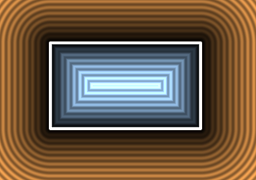
\includegraphics[width=0.38\linewidth]{images/sdf.png}
	\caption{Ilustracija funkcije udaljenosti \cite{sdf}}
	\label{slk:sdf}
\end{figure}

\section{Fraktali}
Najčešće se koristi matematički zapis za opis jednostavnih oblika kao ravnine, sfere ili trokuta. Ako pokušavamo matematički opisati neki kompleksniji oblik kao na primjer zec, brzo postane očito da će to biti vrlo teško. Može se pretpostaviti da je kompleksnost formule raste s kompleksnosti oblika. No, to nije uvijek slučaj. Ispada da jednostavna formula može napraviti vrlo detaljan oblik, a najbolji primjer toga su fraktali. Fraktali su objekti sa svojstvom samoponavljanja. Odnosno, postoji uzorak (ili \emph{pattern}) koji se ponavlja po modelu, na raznim mjestima i raznim veličinama. Ponavljanje tog uzorka može ići do beskonačnosti, što znaći da je fraktal u teoriji ima beskonačno detalja. Ovdje funkcije daljine imaju koristi jer se mogu korisiti za opis fraktala.

\newpage{}

\section{Algoritam iscrtavanja}
Cilj je postići prikaz fraktala. Potreban je algoritam koji uzima opis tijela u obliku funkcije u daljenosti i iscrtava trodimenzionalni prikaz tog tijela na ekranu. Koristiti će se metoda praćenja sfere, što je podvrsta metode koračenja zrake, što je još podvrsta metode praćenja zrake. Metoda praćenja zrake (\emph{engl. Ray Tracing}) određuje boju svakog piksela pomoću zrake koja počinje u očištu kamere i prolazi kroz taj piksel. Metoda koračenja (\emph{engl. Ray Marching}) zrake koristi definiranu zraku tako da postepeno korači u smjeru zrake tijekom računanja. Praćenje sfere (\emph{engl. Sphere Tracing}) dalje definira koračenje tako da je duljina svakog koraka određena na temelju funkcije udaljenosti. Prikazivanjem svakog skoka i pripadajuće vrijednosti udaljenosti se dobiva slika sfera (ili kružnica ako se gleda u 2D prostoru), što se može vidjeti na slici \ref{slk:spheretracing}.

\begin{figure}[htb]
	\centering
	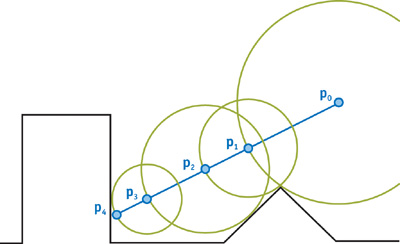
\includegraphics[width=0.38\linewidth]{images/spheretracing.jpg}
	\caption{Koraci zrake u praćenju sfere \cite{spheretracing}}
	\label{slk:spheretracing}
\end{figure}

Ispod je naveden pseudo-kod (Algoritam \ref{alg:spheretracing}) koji prikazuje postupak metode praćenja sfere. U svakoj iteraciji petlje se računa udaljenost pomoću funkcije udaljenosti i obavi se korak duljine te udaljenosti u smjeru zrake. Petlja završava kada je zraka dotaknula tijelo ili kada prođe granicu maksimalnog broja koraka. Mora se zadati granica koraka zbog slućaja kada zraka ne udari tijelo, nego nastavi koračiti u beskonačnost. Zbog nepreciznosti brojeva s pomičnim zarezom može doći do slučaja da zraka nikada ne dođe do udaljenosti nula od tijela. Pritom se za uvjet dodira dodaje varijabla \emph{epsilon}, koja ima vrijednost vrlo malog broja. 

% \begin{lstlisting}
% function pracenje_sfere(org, dir, max, epsilon)
% 	// org - ishodiste zrake
% 	// dir - smjer zrake
% 	// max - maksimalan broj koraka
% 	// epsilon - vrlo mali broj
% 	pos = org
% 	dist = +infinity
% 	count = 0
% 	while (dist > epsilon and count < max)
% 		dist = sdf(pos)
% 		pos += dir * dist
% 		count += 1
% 	return pos
% \end{lstlisting}

\begin{algorithm}[H]
    \caption{Praćenje sfere}
	\label{alg:spheretracing}
    \Fn{pracenjeSfere(org, dir)}{
		\tcp{org - ishodiste zrake}
		\tcp{dir - smjer zrake}
		\tcp{max - maksimalan broj koraka (globalna varijabla)}
		\tcp{epsilon - vrlo mali broj (globalna varijabla)}
		pos = org\;
		dist = $\infty$\;
		count = 0\;
		\While{(dist > epsilon and count < max)}{
			dist = sdf(pos)\;
			pos += dir * dist\;
			count += 1\;
		}
		\Return{pos}
    }
\end{algorithm}

\chapter{Implementacija}
\label{pog:implementacija}

\section{Korišteni alati}

Primarni alat koji je korišten za ovaj rad je biblioteka WebGL2. To je varijanta popularne grafičke biblioteke OpenGL koja je prilagođena za rad na internetskom pregledniku i jeziku \emph{JavaScript}. Mogućnost korištenja grafičkih funkcija na internetskom pregledniku ima mnoge prednosti: omogućuje kompleksne vizualizacije unutar web stranica, izradu video igara koje su dostupne bez instaliravanja izvršne datoteke i generalni pristup procesorne moći grafićke kartice unutar JavaScript. WebGL2 nije sasvim identičan OpenGL, jedna bitna razlika je što ne omogućuje izradu računskih sjenčara (\emph{engl. compute shaders}). Takvi sjenčari su pogodni za iscrtavanje temeljenom zrakama kao praćenje sfera, no moguće je izvesti takvo iscrtavanje koristeći sjenčare fragmenta.

Kao što je već spomenuto, programski jezik koji se koristi je JavaScript. JavaScript ima svojih prednosti što se tiće grafićkih aplikacija. Zajedno s \emph{HTML} i \emph{CSS} pruža jednostavan i fleksibilan način izrade korisničkog sučelja za upravljanje programom. Implementacija grafičkih sučelja u drugim jezicima kao C++ bi bila znatno teža i bilo bi potrebno koristiti datoteke kao na primjer Dear ImGui \cite{imgui}, što ima manju fleksibilnost u dizajnu. Dodatno, web aplikacije su orijenirane na portabilan dizajn na način da jedna stranica može raditi na više vrsta uređaja. To uključuje i ovaj projekt: prikaz fraktala se može otvoriti na mobitelu, a sučelje se prilagođava na orijentaciju i veličinu ekrana. Naravno, kvaliteta i brzina iscrtavanja će ovisiti o grafičkom procesoru uređaja na kojem se izvodi.

\newpage{}

\section{Komponente programa}

Ovo poglavlje služi za kratak opis glavnih dijelova programa. To su četiri klase, koje se zajedno sa svim ostalim klasama, nalaze u dijagramu razreda. Klasa \textbf{\emph{Renderer}} upravlja svim ostalim dijelovima: poziva inicijalizaciju scene i sučelja, učitava pohranjene postavke i upravlja komunikacijom između objekata. Zatim je klasa \textbf{\emph{GPUManager}}, koja je najkompleksnija. Stvara WebGL2 kontekst, poziva WebGL2 funkcije, upravlja sjenčarima, sinkronizira rezoluciju ekrana i definira kako će se izvršiti postupak iscrtavanja okvira (detaljnije u sljedećem poglavlju). Klasa \textbf{\emph{GUIManager}} implementira funkcionalnosti korisničkog sučelja tako da pri učitavanju stranice sagradi sučelje i aktivno ažurira uniformne varijable sjenčara kada se korisnik promijeni vrijednosti. Konačno je zadnja glavna klasa \textbf{\emph{Camera}}. Kamera služi kao kontejner informacija potrebnih za inicijalizaciju zraka i uređuje te podatke na temelju korisničkih ulaza tipkovnicom i mišem.

\todo{graf}

\newpage{}

\section{Postupak iscrtavanja}

Iscrtavanje je stvaranje slike koja se prikaže na ekranu. Za virtualne scene s ciljem prikaza u stvarnom vremenu, frekvencija iscrtavanja mora biti dovoljno velika. Radi brzine, veliki dio postupka iscrtavanja je izveden hardverski i postoji definirani grafički protočni sustav kojeg se treba pridržavati da bi se nacrtao neki 3D model. Trodimenzionalni model prvo prolazi kroz geometrijsku fazu, a zatim rastersku fazu prije popunjavanja okvira. U WebGL2 je ta struktura obavezna, odnosno nije moguće izvršiti crtanje bez pripadajueg sjenčara geometrije (\emph{engl. vertex shader}) i sjenčara fragmenata (\emph{engl. fragment shader}). U ovome slučaju, modeli koje želimo prikazati se ne sastoje od trokuta i nije potrebna geometrijska faza i bilo najbolje koristiti računske sjenčare. No, kao što je prije navedeno, WebGL2 ne omogućuje izradu računske sjenčare. Stoga je postupak iscrtavanja izveden onime što imamo.

Crtanje okvira se izvodi u dva poziva na crtanje (\emph{engl. draw calls}). U svakom pozivu na crtanje se izvodi standardna grafička protočna struktura za WebGL2: sjenčar geometrije se iterira po točkama modela i sjenčar fragmenata se iterira po fragmentima. Jedini model kojeg koristimo je kvadrat (od dvoje trokuta) koji pokriva cijeli ekran. Taj model i geometrijski sjenčar se koriste za oba poziva za crtanje. Prvo iscrtavanje izvodi algoritam praćenje sfere i boji piksele. Rezultat ne ide u standardnu slikovnu prikaznu memoriju (\emph{engl. color buffer}), nego se sprema u privremeni spremnik. Privremeni spremnik ima svojeg para koji zajedno čine takozvani \emph{ping-pong buffer}.

\todo{graf}

\section{Korisničko sučelje}
\todo{vrste inputa, kontrole, mobilno}

\section{Prikaz funkcija udaljenosti}

\subsection{Unos funkcije}
\todo{jezik, funkcije, errori}
\todo{kako radi}

\subsection{Ponuđeni fraktali}
\todo{mandelbox, mandelbulb, koch curve, julia bulb}
\todo{slike}

\subsection{Načini prikaza}
\todo{marches, normal, phong, pathtracing}
\todo{slike}

\section{Web stranica i izvorni kod}

Izvorni kod rada se nalazi na \emph{GitHub} repozitoriju preko sljedeće poveznice: \newline
\url{https://github.com/martzin23/webgl2-fractal-raymarcher}

Aplikacija se izvodi na web pregledniku i kompatabilna je s mobilnim uređajima. Bitno je naglasiti da program neće ispravno raditi ako uređaj ili web preglenik ne podržavaju sve WebGL2 značajke koje se koriste. Aplikacija je dostupna na navedenoj poveznici: \newline
\url{https://martzin23.github.io/webgl2-fractal-raymarcher/}

%--- REZULTATI I RASPRAVA ----------------------------------------------------------------------------

\chapter{Rezultati i rasprava}
\label{pog:rezultati_i_rasprava}
\todo{kvaliteta}
\todo{performanse}
\todo{slike}

%--- ZAKLJUČAK / CONCLUSION ----------------------------------------------------

\chapter{Zaključak}
\label{pog:zakljucak}
\todo{zakljucak}

%--- LITERATURA / REFERENCES ---------------------------------------------------

% Literatura se automatski generira iz zadane .bib datoteke / References are automatically generated from the supplied .bib file
% Upiši ime BibTeX datoteke bez .bib nastavka / Enter the name of the BibTeX file without .bib extension
\bibliography{dependencies/literatura}

%--- SAŽETAK / ABSTRACT --------------------------------------------------------

% Sažetak na hrvatskom
\begin{sazetak}
  \todo{Unesite sažetak na hrvatskom.}
\end{sazetak}

\begin{kljucnerijeci}
  fraktali; WebGL2; koračenje zrakom; praćenje sfera; funkcija daljine
\end{kljucnerijeci}

% Abstract in English
\begin{abstract}
  \todo{Enter the abstract in English.}
\end{abstract}

\begin{keywords}
  fractals; WebGL2; ray marching; sphere tracing; signed distance function
\end{keywords}

%--- PRIVITCI / APPENDIX -------------------------------------------------------

% Sva poglavlja koja slijede će biti označena slovom i riječi privitak / All following chapters will be denoted with an appendix and a letter
% \backmatter

% \chapter{The Code}
% [???]

\end{document}
